%% This document shows an example of writing exam paper in a single file.
%%
\documentclass[12pt]{article}
%\usepackage{finalxm}			% usually final exam. solid hours without minutes
\usepackage[minutes]{finalxm}	% show hours & minutes
%\usepackage[answers]{finalxm}	% answer scheme
%\usepackage{pdflscape}	% for landscape layout on specific page 

\usepackage{lipsum}

\usepackage{amsmath}
\usepackage{amssymb}% for \mathbb

%\usepackage{mathptmx}
%\usepackage{mathpazo}


% Declare graphics path 
 \graphicspath{{./Figures/}}	% a subfolder named figs

%%%%%%%%%%%%%%%%%%%%%%%%%%%
%%% PERSONALIZED STYLES %%%
%%%%%%%%%%%%%%%%%%%%%%%%%%%

%% WITH CAPTION %%
%% Options availabe for caption. put these before begin{figure/table}
%% font, labelfont, textfont || use either bf, normalfont
%% labelsep || use either newline, colon
%\captionsetup[figure]{labelsep=newline, font=normalfont} 	% all bold
%\captionsetup[table]{labelsep=newline, font=normalfont}	% all bold
%\captionsetup[figure]{labelsep=colon} 	% all bold
%\captionsetup[table]{labelsep=colon}	% all bold
%\captionsetup[figure]{labelsep=colon, textfont=normalfont} 	% bold Figure
%\captionsetup[table]{labelsep=colon, textfont=normalfont} 	% bold Table
%\captionsetup[figure]{labelsep=colon, font=normalfont} 	% all no bold 
%\captionsetup[table]{labelsep=colon, font=normalfont} 	% all no bold 

%%%%%%%%%%%%%%%%%%%%%%%%
%%% SETUP TITLE PAGE %%%
%%%%%%%%%%%%%%%%%%%%%%%%
\mtefe{Akhir} 			% Akhir, Pertengahan 
\semester{Kedua}		% Pertama, Kedua
\sidang{2018/2019}		
\examMonthYear{Jun 2019}
\courseCode{ENT342}
\courseNameEn{Computational Fluid Dynamics}
\courseNameBM{Pengiraan Dinamik Bendalir}
\pagesbm{TIGA PULUH SATU}	% used if the number of pages exceeds 30
\durationhr{3 Jam}		% duration of exam
\makeatletter 
%\if@minutes
%	\durationmin{30 Minit}	% MUST be enabled using \usepackage[minutes]{finalxm}
%\fi 		
\makeatother		

%test
\DeclareMathAlphabet{\mathpzc}{OT1}{pzc}{m}{it}

\begin{document}
\makecover	% make cover/title page

\instructionen{
	This question paper has \textbf{FIVE (5)} questions. Answer \textbf{ALL} questions in \textbf{PART A} and any \textbf{ONE (1)} questions in \textbf{PART B}. Each question contributes 25 marks.%
}
\instructionbm{%
	Kertas soalan ini mengandungi \textbf{LIMA (5)} soalan. Jawab \textbf{semua} soalan di \textbf{BAHAGIAN A} dan mana-mana \textbf{SATU (1)} soalan di \textbf{BAHAGIAN B}. Markah bagi setiap soalan adalah 25 markah.%
}

%Note: Some tables and equations are given in the Appendix
%[Nota : Beberapa jadual dan persamaan diberikan dalam Lampiran]

% Delete from here if require no extra notes 
%\vskip 3em
%\instructionen{
%	Note: Tables and equations are given in the Appendix.%
%}
%\instructionbm{%
%	Nota: Jadual dan persamaan diberi dalam Lampiran.%
%}
% Delete until here if require no extra notes 

\makecoverend	% end cover/title page

%%%%%%%%%%%%%%%%%%%%%%%%%%%%
%%% MAIN BODY START HERE %%%
%%%%%%%%%%%%%%%%%%%%%%%%%%%%
\setmainstyle
\vskip -2em		% adjust vertical space skip accordingly 

%%%%%%%%%%%%%
%%% PART  %%%
%%%%%%%%%%%%%
%\textbf{Answer all questions} 
%
%\translationbf{Jawab semua soalan}
%\bigskip
 \newparten{Answer all questions}

\newpartbm{Jawab semua soalan}


%%%%%%%%%%%%%%%%%%
%%% QUESTION 1 %%%
%%%%%%%%%%%%%%%%%%
%TODO Question1
 \bigskip 
%\partQuestion{[CO1, PO1]}

%\setmainstyle
%\vskip -2em		% adjust vertical space skip accordingly 

%%%%%%%%%%%%%
%%% PART  %%%
%%%%%%%%%%%%%
%\textbf{Answer all questions} 
%
%\translationbf{Jawab semua soalan}
%\bigskip
%\newparten{Answer all questions}

%\newpartbm{Jawab semua soalan}


%%%%%%%%%%%%%%%%%%
%%% QUESTION 1 %%%
%%%%%%%%%%%%%%%%%%
%TODO Question1
%\bigskip 

\question{}[\label{q1}]

The governing equations for inviscid compressible flow is the Euler equations. The equations can be derived from three conservations principle which are the mass conservation, momentum conservation and energy conservation. The principles can be easily demonstrated for one-dimensional flow. Answer the questions below regarding the one-dimensional Euler equations.

\translation{Persamaan menakluk untuk aliran tidak likat boleh mampat adalah persamaan Euler. Persamaan ini boleh diterbitkan daripada tiga prinsip keabadian iaitu prinsip keabadian untuk jisim, momentum dan tenaga. Prinsip-prinsip ini dapat ditunjukkan dengan mudah untuk aliran satu dimensi. Jawab soalan-solan dibawah berkaitan dengan persamaan Euler satu dimensi.}

\listbeginx	% start 1st level question
	\item \label{item:q1a} Explain the three principle of conservations and their relations to the control volume analysis. Sketch a suitable control volume for your explanation.
	
	\translation{Jelaskan tiga prinsip keabadian itu dan hubungannya dalam analisa isipadu kawalan. Lakarkan rajah isipadu kawalan yang sesuai untuk penjelasan anda.} 

\qmarks{10}	
	
	\item \label{item:q1b} Using the information from Q\ref{q1}\ref{item:q1a}, prove that the one-dimensional Euler equations can be written in the form below. Here, $\rho$, $u$, $p$, $e$ are density, x-axis velocity, pressure and total energy, respectively.
		
		\translation{Dengan menggunakan maklumat daripada Q\ref{q1}\ref{item:q1a},buktikan bahawa persamaan Euler satu dimensi boleh ditulis dalam bentuk dibawah. Disini, $\rho$, $u$, $p$, $e$ adalah masing-masingnya ketumpatan, halaju pada paksi-x, tekanan dan tenaga keseluruhan.  }
	
	\begin{equation}
	\frac{\partial \textbf{Q} }{\partial t} + \frac{\partial \textbf{E}}{\partial x} = 0 \nonumber
	\end{equation}
	
	\begin{equation}
	\textbf{Q} = \begin{bmatrix}
	\rho \\ \rho u \\ e
	\end{bmatrix}    \nonumber
\end{equation}

\begin{equation}	
	\textbf{E} = \begin{bmatrix}
\rho u \\ \rho u^2 + p \\ (e+p)u
\end{bmatrix}	\nonumber
	\end{equation}
		
		
		\qmarks{10}

\item There are \textbf{four (4)} unknown variables in the equations from Q\ref{q1}\ref{item:q1b} but only \textbf{three (3)} equations, meaning that the system needs another equation to close it. The pressure $p$ and total energy $e$ are linked together by the state equation of ideal gas. Demonstrate the relation between the two quantities.

\translation{Terdapat empat (4) anu dalam kesemua persamaan daripada Q\ref{q1}\ref{item:q1b} tetapi cuma tiga (3) persamaan, bermakna sistem persamaan ini memerlukan satu lagi persamaan untuk dipenuhi. Tekanan $p$ dan tenaga keseluruhan $e$ adalah berkaitan dengan persamaan keadaan untuk gas unggul. Tunjukkan hubungan antara kedua-dua kuantiti itu.}		
		
		\qmarks{5}
\listclose % close 1st level question


%%%%%%%%%%%%%%%%%%
%%% QUESTION 2 %%%
%%%%%%%%%%%%%%%%%%
%TODO Question2
\clearpage		% page break
\question{}
%\partQuestion{}

The Marker-and-Cell (MAC) algorithm belongs to a group of solution algorithm called \textit{pressure correction} method for incompressible Navier-Stokes equations. The incompressible Navier-Stokes equations are given below in differential form where $\textbf{u}$, p and $\nu$ are velocity vector, pressure and dynamic viscosity coefficient, respectively. The MAC algorithm closes the system equations by using the mass conservation equation or divergence equation to link the pressure with velocity gradients. Answer the questions below regarding the MAC algorithm.   

\translation{Algoritma Penanda-dan-Sel (MAC) termasuk didalam satu kumpulan algoritma solusi yang dipanggil kaedah \textit{pembetulan tekanan} untuk persamaan tidak mampat Navier-Stokes. Persamaan tidak mampat Navier-Stokes diberikan seperti dibawah dimana $\textbf{u}$, p dan $\nu$ masing-masing adalah vektor halaju, tekanan dan pekali kelikatan dinamik. Algoritma MAC menutup sistem persamaan ini dengan menggunakan persamaan keabadian jisim atau persamaan mencapah yang dikaitkan dengan tekanan dan kecerunan halaju. Jawab soalan-soalan dibawah berkenaan algoritma MAC}

\begin{subequations}
\begin{align}
\nabla \cdot \textbf{u} &= 0 \nonumber  \\ \nonumber
\frac{\partial \textbf{u}}{\partial t} + \textbf{u} \cdot \nabla \textbf{u}  &= -\nabla p + \nu \nabla^2 \textbf{u},
\end{align}
\end{subequations}

\listbeginx	% start 1st level question
	\item Explain the step-by-step of MAC algorithm using the incompressible Navier-Stokes equations given. Give the supporting mathematical argument for each step.  	
	
	\translation{Terangkan langkah-langkah penyelesaian persamaan tidak mampat Navier-Stokes menggunakan algoritma MAC. Berikan sokongan matematik bagi setiap langkah-langkah tersebut.}
	
		
		\qmarks{10}
	
%	\nextpage 
%	\clearpage 
	
	\item The staggered grid configuration is very effective in removing checkered pressure field solution. For this reason, the MAC algorithm applied the staggered grid configuration in its early inception. Construct the staggered grid configuration for two-dimensional structure and propose how to discretize the differential terms $\frac{\partial u}{\partial x}$, $\frac{\partial u}{\partial y}$ and $\frac{\partial p}{\partial x}$ for the given grid.       

	\translation{Konfigurasi grid tidak serentak sangat berkesan untuk menyahkan solusi medan tekanan berkotak. Oleh sebab itu, pada awal-awalnya algoritma MAC telah menggunakan konfigurasi grid tidak serentak ini. Binakan grid tidak serentak untuk struktur dua dimensi dan berikan cadangan bagaimana terma-terma pembezaan $\frac{\partial u}{\partial x}$, $\frac{\partial u}{\partial y}$ dan $\frac{\partial p}{\partial x}$ boleh didiskretkan untuk grid tersebut.}
	

\qmarks{10}	
	

\item Can the checkered pressure field solution be avoided using normal grid? Analyze the problem to determine the cause.
	
	\translation{Bolehkah penyelesaian medan tekan berpetak dielak menggunakan grid normal? Analisa masalah itu untuk menentukan puncanya.}

\qmarks{5}



\listclose	% close 1st level question



%TODO PART B
\clearpage
\newpartenx{Answer TWO (2) questions ONLY}

\newpartbm{Jawab DUA (2) soalan SAHAJA}
\bigskip 

%\question{}
%\partQuestion{}

%%%%%%%%%%%%%%%%%%
%%% QUESTION 3 %%%
%%%%%%%%%%%%%%%%%%
%TODO Question3
%\clearpage		% page break
\question{}\label{q3}
%\partQuestion{}

The one-dimensional linear advection equation is the canonical example of transport phenomena. The equation is an excellent model equation to test the behavior of numerical method. The equation is given as below.  
	
	\translation{Persamaan adveksi linear satu dimensi merupakan satu contoh persamaan berkanun bagi fenomena pengangkutan. Persamaan ini juga merupakan satu persamaan model yang sangat cemerlang untuk menguji sifat-sifat kaedah berangka. Persamaan ini diberikan seperti dibawah.}
	
	\begin{equation}
	\frac{\partial u}{\partial t} + c \frac{\partial u}{\partial x} = 0, \quad c > 0 \nonumber
	\end{equation}		

\listbeginx	% start 1st level question			

    \item \label{q3a} The finite volume method can be applied to numerically solve the linear advection equation. Answer the question below regarding the finite volume method.	
	\translation{Kaedah isipadu terhingga boleh digunakan untuk menyelesaikan persamaan adveksi linear secara berangka. Jawab soalan-soalan dibawah berkenaan kaedah isipadu terhingga.}

\listbegin
\item \label{q3a1} Apply the finite volume method to derive the semi-discrete form of the advection equation.

\translation{Gunakan kaedah isipadu terhingga untuk menerbitkan persamaan separa-diskrit untuk persamaan adveksi tersebut.}

\qmarks{5}

\item \label{q3a2} Considering a uniform control volume, analyze the possible discretization method for the semi-discrete equation in Q\ref{q3}\ref{q3a}\ref{q3a1}.

\translation{Dengan menganggap isipadu kawalan yang sekata, analisa kaedah diskrit yang mungkin digunapakai untuk persamaan separuh diskrit Q\ref{q3}\ref{q3a}.}

\qmarks{5}

\listclose

		
	\item \label{q3b} From the discrete equation in Q\ref{q3}\ref{q3a}, analyze the numerical stability condition using complex Fourier analysis.   
	
	\translation{Daripada persamaan diskrit Q\ref{q3}\ref{q3a}, analisa syarat kestabilan berangka menggunakan nombor kompleks Fourier.}

	\qmarks{10}
		
	\item What is the conclusion from Q\ref{q3}\ref{q3b}? Is the method stable? Propose a solution if the method is not stable.   
	
	\translation{Apakah kesimpulan daripada Q\ref{q3}\ref{q3b}? Adakah kaedah ini stabil? Cadangkan satu penyelesaian jika kaedah ini tidak stabil.}

	\qmarks{5}

\listclose	% close 1st level question

%%%%%%%%%%%%%%%%%%
%%% QUESTION 4 %%%
%%%%%%%%%%%%%%%%%%
%TODO Question4
\clearpage		% page break
\question{}\label{q4}
%\partQuestion{}


		\begin{figure}[H] % H means, to put figure here after the code
		\centering
		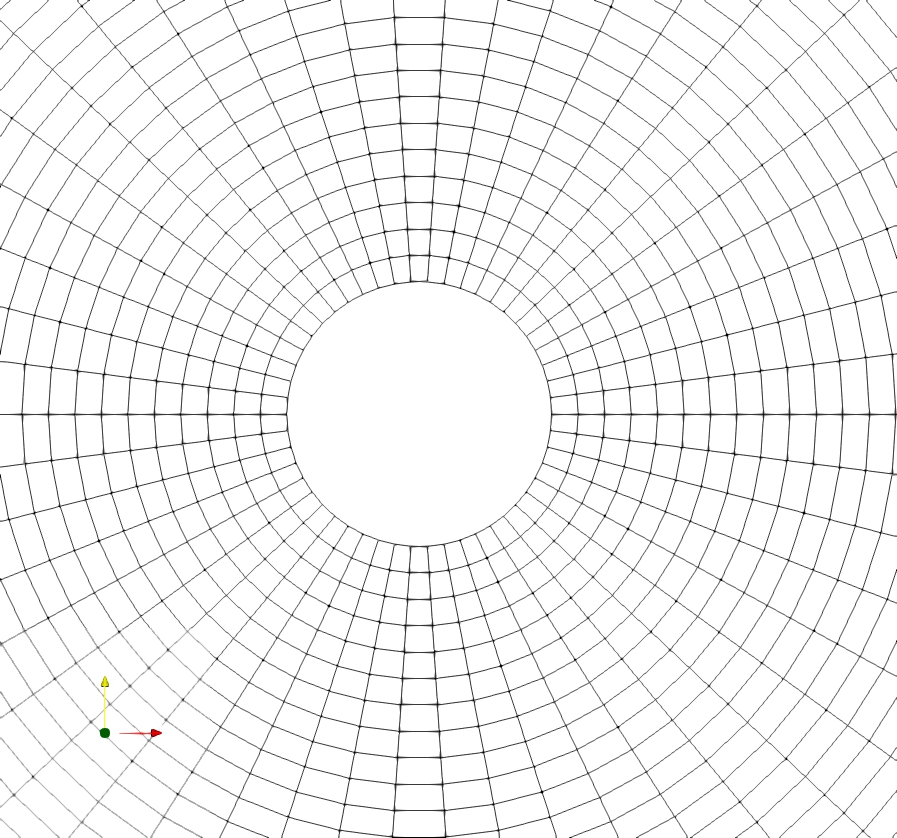
\includegraphics[width=0.75\textwidth, height=0.5\textwidth]{cylinderGrid-1}
		\caption{\rajah}
		\label{fig:cylinder}
	    \end{figure}	

The curvilinear boundary fitted grid as shown in \textbf{Figure \ref{fig:cylinder}}
is generated analytically using the equations below with $r_{0}$ as the radius of the cylinder. Answer the questions below regarding coordinate transformation.

\translation{Grid melengkung padanan sempadan yang ditunjukkan pada Rajah \ref{fig:cylinder} dijana secara analitik menggunakan persamaan dibawah dimana $r_{0}$ merupakan jejari silinder tersebut. Jawab soalan-soalan dibawah berkaitan transformasi kordinat.}

\begin{subequations}
\begin{align}
x(r, \theta) &= (r_{0} + r) \cos \theta \nonumber  \\ \nonumber
y(r, \theta) &= (r_{0} + r)\sin \theta
\end{align}
\end{subequations}
		
\listbeginx	% start 1st level question

\item For each coordinate, the metrics are given as $x_{r}$, $y_{r}$, $x_{\theta}$ and $y_{\theta}$, where the subscript refers to partial derivatives. These metrics are required to transform any physical quantity derivative, for example $u_{x}$, into the computational domain derivatives of $u_{r}$ and $u_{\theta}$. Construct the projection of $u_{x}$ into domain $(r, \theta)$ using the metrics and $(u_{r},u_{\theta})$. 

\translation {Untuk setiap koordinat, metrik-metrik diberikan sebagai $x_{r}$, $y_{r}$, $x_{\theta}$ dan $y_{\theta}$, dimana subskrip merujuk kepada terbitan separa. Metrik-metrik ini diperlukan untuk mengubah apa-apa terbitan kuantiti fizik seperti $u_{x}$ untuk terma terbitan di domain pengiraan $u_{r}$ dan $u_{\theta}$. Binakan unjuran $u_{x}$ ke domain $(r, \theta)$ menggunakan metrik-metrik dan $(u_{r},u_{\theta})$.}
		
\qmarks{10}

\clearpage
%\nextpage

\item \label{q4b} \textbf{Table \ref{table:cell}} shows a sample coordinate of a cell from the grid in \textbf{Figure \ref{fig:cylinder}}. The Jacobian metric, $\textbf{J}$ of any cell in the grid is given as the equation below. Calculate the area of the cell and interpret its relation to the Jacobian metric.

\translation {Jadual\ref{table:cell} menunjukkan sampel koordinat satu sel daripada grid seperti di Rajah\ref{fig:cylinder}. Metrik Jacobian $\textbf{J}$ bagi mana-mana sel dalam grid diberikan seperti persamaan di bawah. Kirakan luas kawasan sel tersebut dan interpretasikan hubungannya dengan metric Jacobian.}

\begin{equation}
\textbf{J} = \det\begin{pmatrix} x_{r} & y_{r} \\ x_{\theta} & y_{\theta}  \end{pmatrix} = x_{r}y_{\theta} - x_{\theta}y_{r} \nonumber
\end{equation}

\listbegin
\item Calculate the area of the cell.

\translation{Kirakan keluasan sel tersebut.}

\qmarks{5}

\item What is the interpretation of the Jacobian metric for the cell area?

\translation{Apakan interpretasi metric Jacobian terhadap keluasan sel tersebut.}

\qmarks{5}

\listclose
				
%\qmarks{10}


\item Sketch the cell in Q\ref{q4}\ref{q4b} roughly and analyze the outward pointing unit normal vector on each of the cell's side.

\translation {Lakarkan secara kasar sel daripada Q\ref{q4}\ref{q4b} dan analisakan vektor unit normal di setiap sisi sel.}
		
\qmarks{5}


\listclose	% close 1st level question

\renewcommand{\arraystretch}{1.2}	% to make better spacing between rows
\begin{table}[H]
	\centering
	\caption{\jadual}	% no caption
	%	\begin{tabularx}{220pt}{c c}
	\begin{tabular}{|c|c|}
		%\toprule
		\hline
		%\toprule[1.5pt]
		\multicolumn{1}{|l|}{\textbf{x}} & \multicolumn{1}{l|}{\textbf{y}} \\
		\hline
0.927051 & 2.85317 \\
0.562144 & 2.94686 \\
0.988854 & 3.04338 \\
0.59962 & 3.14332 \\
		\hline
		%\bottomrule
		%\bottomrule[1.5pt]
	\end{tabular}
	%		\end{tabularx}%
	\label{table:cell}%
\end{table}%


\clearpage
%%%%%%%%%%%%%%%%%%
%%% QUESTION 5 %%%
%%%%%%%%%%%%%%%%%%
%TODO Question5
% \clearpage		% page break
\question{} \label{q5}
%\partQuestion{}

	The time-dependent one-dimensional heat equation is a second-order partial differential equation. The second-order term infers that the solution propagation will be restricted to the order of $O$ $(1/\Delta h^{2})$, where $\Delta h$ is the mesh spacing. This put a severe stability restriction to explicit numerical scheme when solving this equation. Answer the questions referring to the time-dependent one-dimensional heat equation below.
	
	\translation{Persamaan haba satu-dimensi bersandar masa merupakan persamaan kebezaan separa darjah kedua. Terma darjah kedua bererti propagasi solusi disekat pada darjah $\mathcal{O}(1/\Delta h^{2})$, dimana $\Delta h$ adalah jarak antara grid. Ini menyebabkan penyekatan syarat kestabilan yang teruk bagi kaedah berangka tersurat ketika menyelesaikan persamaan ini. Jawab soalan-soalan berkaitan dengan persamaan haba satu-dimensi bersandar masa dibawah.}

\begin{equation}
\frac{\partial T}{\partial t} = \kappa \left( \frac{\partial^2 T}{\partial x^2} \right) \nonumber
\end{equation}		
		
		\listbeginx

\item \label{q5a} Construct the discretized equation for the heat equation using \textit{forward} Euler time integration and centered difference scheme for the spatial term. Analyze the discrete equation to derive the numerical stability condition.

\translation {Bina persamaan diskrit untuk persamaan haba itu menggunakan kaedah integrasi masa Euler kehadapan dan kaedah pembezaan pertengahan untuk terma ruang. Analisakan persamaan diskrit itu untuk menerbitkan syarat kestabilan berangka.}
		
\qmarks{10}

\item \label{q5b} From the discrete equation obtained in Q\ref{q5}\ref{q5a} the time integration scheme can be modified by setting the time step forward or backward. Answer the questions below regarding backward time step method.     

\translation{Daripada persamaan diskrit yang diperolehi oleh Q\ref{q5}\ref{q5a} kaedah integrasi masa boleh diubahsuai dengan menetapkan langkah masa kehadapan atau mundur. Jawab soalan-soalan dibawah berkenaan kaedah mundur langkah masa.}

\listbegin
\item Apply the \textit{backward} Euler time integration to the discrete equation obtained in Q\ref{q5}\ref{q5a} and rearrange the equation.

\translation{Applikasikan kaedah integrasi masa mundur Euler keatas persamaan diskrit yang diperolehi daripada Q\ref{q5}\ref{q5a} dan susun semula persamaan itu.}

\qmarks{5}

\item Analyze the stability condition for the backward Euler time integration.

\translation{Analisakan syarat kestabilan kaedah integrasi masa mundur Euler.}

\qmarks{5}

\listclose

	
	\item The discrete equation from Q\ref{q5}\ref{q5b} contains more unknown at the next time step than at the previous time step. This condition necessitates the construction of simultaneous linear equations. Construct the matrix-vector form for the simultaneous linear equations.  
	
	\translation{Persamaan diskrit daripada Q\ref{q5}\ref{q5b} mengandungi lebih banyak terma di masa seterusnya daripada masa sebelumnya. Keadaan ini memerlukan pembinaan persamaan linear serentak. Bina persamaan linear serentak itu dalam bentuk matriks-vektor.}

	\qmarks{5}



\listclose	% close 1st level question



\paperend 

%\clearpage

%\paperend %<- included in Q6.tex
%\clearpage
\newpage
\textbf{\underline{Appendices}}
\begin{figure}[H] % H means, to put figure here after the code
\centering
\includegraphics[width=\textwidth]{appendix1}
\label{fig:appendix1}
\end{figure}	

\begin{figure}[H] % H means, to put figure here after the code
\centering
\includegraphics[width=\textwidth]{appendix2}
\label{fig:appendix2}
\end{figure}



\end{document}